\documentclass{beamer}
\usetheme{Madrid}
\usepackage[utf8]{inputenc}
\usepackage[T1]{fontenc}
\usepackage{graphicx}
\usepackage{lmodern}

% Remove controls
\setbeamertemplate{navigation symbols}{}
\beamertemplatetransparentcovered

\title{ Getting Things GNOME! Integration with GNOME Shell}
\author{Baptiste Saleil}
\institute{}
\date{July 29, 2012}

\hypersetup{
      pdfauthor   = {Baptiste Saleil},
      pdftitle    = {GUADEC talk - Summer of Code 2012},
      pdfsubject  = {Getting Things GNOME! integration with GNOME Shell},
      pdfkeywords = {GTG, GNOMEShell, GUADEC, GNOME},
      pdfcreator  = {PDFLaTeX},
      pdfproducer = {PDFLaTeX}
}

\setbeamertemplate{footline}
{
  \leavevmode%
  \hbox{%
  \begin{beamercolorbox}[wd=.222222\paperwidth,ht=2.25ex,dp=1ex,center]{author in head/foot}%
    \usebeamerfont{author in head/foot}\insertshortauthor%~~\beamer@ifempty{\insertshortinstitute}{}{(\insertshortinstitute)}
  \end{beamercolorbox}%
  \begin{beamercolorbox}[wd=.555555\paperwidth,ht=2.25ex,dp=1ex,center]{title in head/foot}%
    \usebeamerfont{title in head/foot}\insertshorttitle
  \end{beamercolorbox}%
  \begin{beamercolorbox}[wd=.222222\paperwidth,ht=2.25ex,dp=1ex,right]{date in head/foot}%
    \usebeamerfont{date in head/foot}\insertshortdate{}\hspace*{2em}
    \insertframenumber{} / \inserttotalframenumber\hspace*{2ex} 
  \end{beamercolorbox}}%
  \vskip0pt%
}

\begin{document}

	\begin{frame}
		\titlepage
		\begin{center}
			
\includegraphics[scale=0.5]{gnome.png}
			\hspace{1cm}
			
\includegraphics[scale=0.4]{gsoc.png}
			\hspace{1cm}
			
\includegraphics[scale=0.4]{sponsored.png}
		\end{center}
	\end{frame}

	% DOCUMENT
	\section{Project}
	\begin{frame}{Project}
		\begin{exampleblock}{Goal}<1->
			\centering Use the power of Getting Things GNOME! \\ with the simplicity of GNOME Shell 
		\end{exampleblock}
		\begin{block}{Getting Things GNOME!}<2->
			\begin{itemize}
				\item Tasks management : Add, Modify, Delete, ...
				\item Synchronization services : Tomboy, Launchpad, ...
			\end{itemize}
		\end{block}
		\begin{block}{GNOME Shell}<3->
			\begin{itemize}
				\item User interface : User friendly, simple, intuitive, ...
				\item Power : Centralized search, calendar pop-down menu, ...
			\end{itemize}
		\end{block}
	\end{frame}
	
	\section{What is done ?}
	\begin{frame}{What is done ?}
		\begin{figure}[!t]
			\centering
			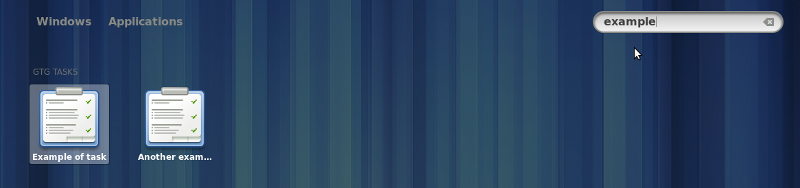
\includegraphics[scale=0.28]{search.png}
			\tiny {\caption{Example of search in overview}}
		\end{figure}
		\begin{figure}[!t]
			\centering
			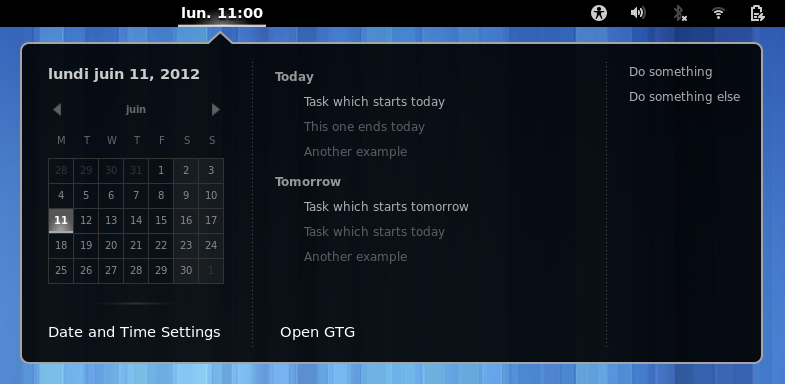
\includegraphics[scale=0.29]{calendar.png}
			\tiny {\caption{Calendar pop-down menu}}
		\end{figure}
	\end{frame}
	
	\begin{frame}{What is done ?}
		\begin{figure}
			\centering
			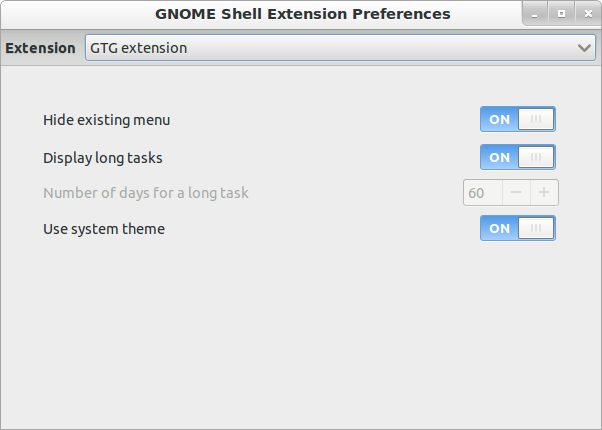
\includegraphics[scale=0.3]{prefs.png}
			\tiny {\caption{Preferences}}
		\end{figure}
	\end{frame}
	
	\begin{frame}{What is planned !}
		\begin{itemize}
			\item Notification system
				\begin{figure}
					\centering
					
\includegraphics[scale=0.3]{notif.png}
					\tiny {\caption{Mockup}}
				\end{figure}
			\item Add preferences
			\item Fix knowing bugs
			\item Improve performance
		\end{itemize}
	\end{frame}
	
	\begin{frame}{}
		
		\begin{block}{Project homepage}<1->
			\centering \textbf{http://bsaleil.org/gtg} \\
			(redirection to live.gnome.org)
		\begin{itemize}
			\item Repository
			\item Blog
			\item ...
		\end{itemize}
		\end{block}
		
		\begin{block}{Thanks to...}<2->
		\begin{itemize}
			\item Luca Invernizzi : My mentor. He helps me for my project, and still here when I have trouble/problem
			\item Gnome foundation : For accepting me to the Summer of Code, and Sponsoring me for GUADEC
		\end{itemize}
		\end{block}
		
		\begin{center}
			\LARGE {\uncover<3->{Thanks for your attention !}}
		\end{center}
	\end{frame}

\end{document}
